%!TEX TS-program = xelatex

% Шаблон документа LaTeX создан в 2018 году
% Алексеем Подчезерцевым
% В качестве исходных использованы шаблоны
% 	Данилом Фёдоровых (danil@fedorovykh.ru) 
%		https://www.writelatex.com/coursera/latex/5.2.2
%	LaTeX-шаблон для русской кандидатской диссертации и её автореферата.
%		https://github.com/AndreyAkinshin/Russian-Phd-LaTeX-Dissertation-Template

\documentclass[a4paper,14pt]{article}


%%% Работа с русским языком
\usepackage[english,russian]{babel}   %% загружает пакет многоязыковой вёрстки
\usepackage{fontspec}      %% подготавливает загрузку шрифтов Open Type, True Type и др.
\defaultfontfeatures{Ligatures={TeX},Renderer=Basic}  %% свойства шрифтов по умолчанию
\setmainfont[Ligatures={TeX,Historic}]{Times New Roman} %% задаёт основной шрифт документа
\setsansfont{Comic Sans MS}                    %% задаёт шрифт без засечек
\setmonofont{Courier New}
\usepackage{indentfirst}
\frenchspacing

\renewcommand{\epsilon}{\ensuremath{\varepsilon}}
\renewcommand{\phi}{\ensuremath{\varphi}}
\renewcommand{\kappa}{\ensuremath{\varkappa}}
\renewcommand{\le}{\ensuremath{\leqslant}}
\renewcommand{\leq}{\ensuremath{\leqslant}}
\renewcommand{\ge}{\ensuremath{\geqslant}}
\renewcommand{\geq}{\ensuremath{\geqslant}}
\renewcommand{\emptyset}{\varnothing}

%%% Дополнительная работа с математикой
\usepackage{amsmath,amsfonts,amssymb,amsthm,mathtools} % AMS
\usepackage{icomma} % "Умная" запятая: $0,2$ --- число, $0, 2$ --- перечисление

%% Номера формул
%\mathtoolsset{showonlyrefs=true} % Показывать номера только у тех формул, на которые есть \eqref{} в тексте.
%\usepackage{leqno} % Нумерация формул слева	

%% Перенос знаков в формулах (по Львовскому)
\newcommand*{\hm}[1]{#1\nobreak\discretionary{}
	{\hbox{$\mathsurround=0pt #1$}}{}}

%%% Работа с картинками
\usepackage{graphicx}  % Для вставки рисунков
\graphicspath{{images/}}  % папки с картинками
\setlength\fboxsep{3pt} % Отступ рамки \fbox{} от рисунка
\setlength\fboxrule{1pt} % Толщина линий рамки \fbox{}
\usepackage{wrapfig} % Обтекание рисунков текстом

%%% Работа с таблицами
\usepackage{array,tabularx,tabulary,booktabs} % Дополнительная работа с таблицами
\usepackage{longtable}  % Длинные таблицы
\usepackage{multirow} % Слияние строк в таблице
\usepackage{float}% http://ctan.org/pkg/float

%%% Программирование
\usepackage{etoolbox} % логические операторы


%%% Страница
\usepackage{extsizes} % Возможность сделать 14-й шрифт
\usepackage{geometry} % Простой способ задавать поля
\geometry{top=20mm}
\geometry{bottom=20mm}
\geometry{left=20mm}
\geometry{right=10mm}
%
%\usepackage{fancyhdr} % Колонтитулы
% 	\pagestyle{fancy}
%\renewcommand{\headrulewidth}{0pt}  % Толщина линейки, отчеркивающей верхний колонтитул
% 	\lfoot{Нижний левый}
% 	\rfoot{Нижний правый}
% 	\rhead{Верхний правый}
% 	\chead{Верхний в центре}
% 	\lhead{Верхний левый}
%	\cfoot{Нижний в центре} % По умолчанию здесь номер страницы

\usepackage{setspace} % Интерлиньяж
\onehalfspacing % Интерлиньяж 1.5
%\doublespacing % Интерлиньяж 2
%\singlespacing % Интерлиньяж 1

\usepackage{lastpage} % Узнать, сколько всего страниц в документе.

\usepackage{soul} % Модификаторы начертания

\usepackage{hyperref}
\usepackage[usenames,dvipsnames,svgnames,table,rgb]{xcolor}
\hypersetup{				% Гиперссылки
	unicode=true,           % русские буквы в раздела PDF
	pdftitle={Заголовок},   % Заголовок
	pdfauthor={Автор},      % Автор
	pdfsubject={Тема},      % Тема
	pdfcreator={Создатель}, % Создатель
	pdfproducer={Производитель}, % Производитель
	pdfkeywords={keyword1} {key2} {key3}, % Ключевые слова
	colorlinks=true,       	% false: ссылки в рамках; true: цветные ссылки
	linkcolor=black,          % внутренние ссылки
	citecolor=black,        % на библиографию
	filecolor=magenta,      % на файлы
	urlcolor=black           % на URL
}
\makeatletter 
\def\@biblabel#1{#1. } 
\makeatother
\usepackage{cite} % Работа с библиографией
%\usepackage[superscript]{cite} % Ссылки в верхних индексах
%\usepackage[nocompress]{cite} % 
\usepackage{csquotes} % Еще инструменты для ссылок

\usepackage{multicol} % Несколько колонок

\usepackage{tikz} % Работа с графикой
\usepackage{pgfplots}
\usepackage{pgfplotstable}

% ГОСТ заголовки
\usepackage[font=small]{caption}
%\captionsetup[table]{justification=centering, labelsep = newline} % Таблицы по правобу краю
%\captionsetup[figure]{justification=centering} % Картинки по центру


\newcommand{\tablecaption}[1]{\addtocounter{table}{1}\small \begin{flushright}\tablename \ \thetable\end{flushright}%	
\begin{center}#1\end{center}}

\newcommand{\imref}[1]{рис.~\ref{#1}}

\usepackage{multirow}
\usepackage{spreadtab}
\newcolumntype{K}[1]{@{}>{\centering\arraybackslash}p{#1cm}@{}}


\usepackage{xparse}
\usepackage{fancyvrb}

\RecustomVerbatimCommand{\VerbatimInput}{VerbatimInput}
{
	fontsize=\footnotesize    
}

\usepackage{tocloft}
\renewcommand{\cftsecleader}{\cftdotfill{\cftdotsep}}
\begin{document} % конец преамбулы, начало документа
\begin{titlepage}
	\begin{center}
 		ФЕДЕРАЛЬНОЕ  ГОСУДАРСТВЕННОЕ АВТОНОМНОЕ \\
		ОБРАЗОВАТЕЛЬНОЕ УЧРЕЖДЕНИЕ ВЫСШЕГО ОБРАЗОВАНИЯ\\
		«НАЦИОНАЛЬНЫЙ ИССЛЕДОВАТЕЛЬСКИЙ УНИВЕРСИТЕТ\\
		«ВЫСШАЯ ШКОЛА ЭКОНОМИКИ»
	\end{center}
	
	\begin{center}
		\textbf{Московский институт электроники и математики}
		
		\textbf{им. А.Н.Тихонова НИУ ВШЭ}
		
		\vspace{2ex}
		
		\textbf{Департамент компьютерной инженерии}
	\end{center}
	\vspace{1ex}	
	
	\begin{center}
	\textbf{ОТЧЕТ\\
		ПО ЛАБОРАТОРНОЙ РАБОТЕ №6
	}
	\end{center}	
	\vspace{2ex}
	\begin{center}
		по дисциплине «Проектирование систем на кристалле»
	\end{center}	

	\vspace{2ex}

	\begin{flushright}
		\textbf{Выполнили:}
		
		\vspace{2ex}
		
		Студенты группы БИВ174
		
		Бригада №5
		
		\vspace{2ex}
		
		Подчезерцев Алексей Евгеньевич
		
		Солодянкин Андрей Александрович
		\vspace{2ex}
		
	\end{flushright}

	\vfill
	\begin{center}
		Москва \the\year \, г.
	\end{center}
	
\end{titlepage}
\addtocounter{page}{1}
\tableofcontents
\pagebreak

\section{Задание}

Создать сумматор-накопитель, входные данные A и B по 8 бит, поступают из RAM. 
По разрешающему сигналу данные складываются и добавляются к предыдущему результату.
Предусмотреть сброс данных в накопителе.

\section{Выполнение работы}

Создадим проект, в качестве device выберем 10M50DCF484C7G семейства MAX 10.

Добавим в проект IP блок двупортовой памяти (рис.~\ref{fig:ram_1}) и настроим его (рис.~\ref{fig:ram_2}).
Также добавим блок параллельного сумматора (рис.~\ref*{fig:add}).

\begin{figure}[H]
	\centering
	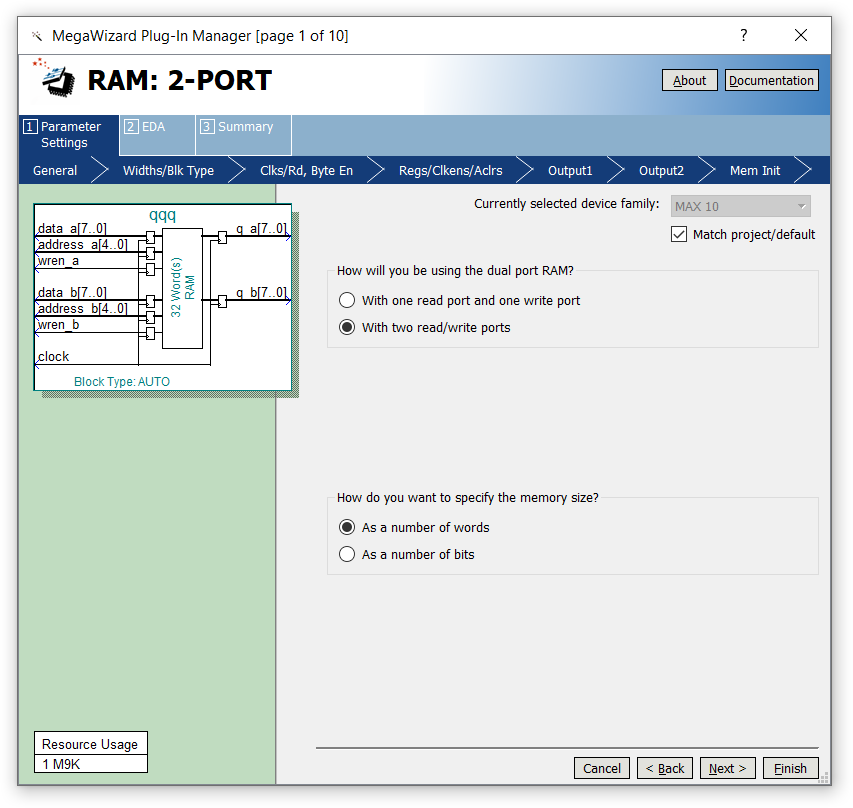
\includegraphics[width=\linewidth]{image/ram_1}
	\caption{Создание блока RAM}
	\label{fig:ram_1}
\end{figure}

\begin{figure}[H]
	\centering
	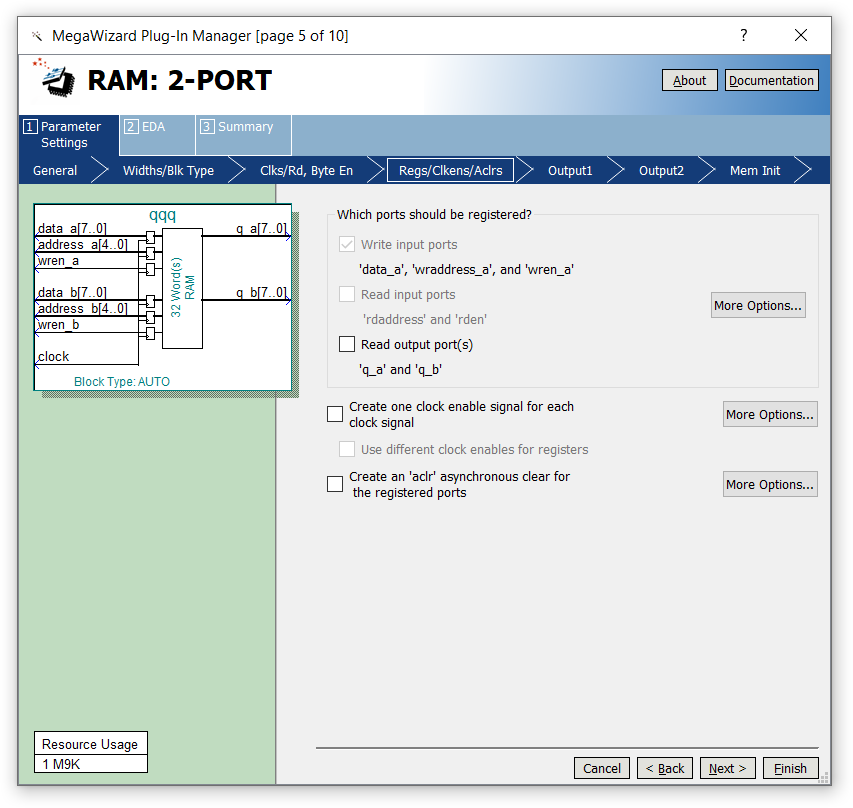
\includegraphics[width=\linewidth]{image/ram_2}
	\caption{Настройка блока RAM}
	\label{fig:ram_2}
\end{figure}

\begin{figure}[H]
	\centering
	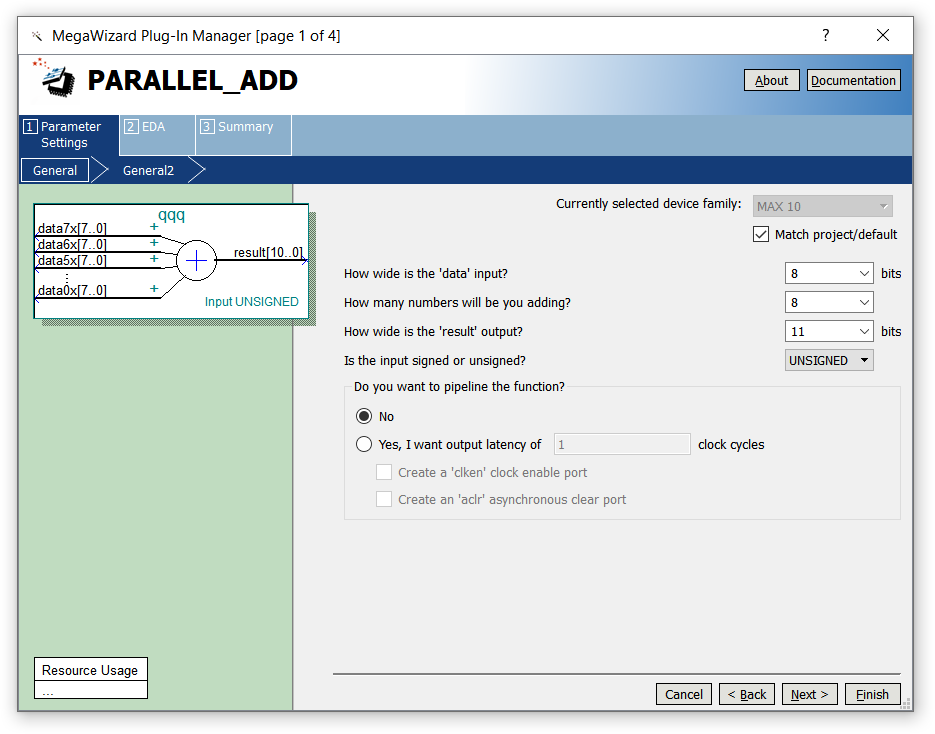
\includegraphics[width=\linewidth]{image/add}
	\caption{Создание блока сумматора}
	\label{fig:add}
\end{figure}

Создадим схему проекта (рис~\ref{fig:schema}).
Входные данные записываются в двупортовую память, оттуда поступают на вход сумматора, результат записывается в триггер и дублируется на вход сумматора.
Предусмотрен сигнал сброса накопленного результата.

\begin{figure}[H]
	\centering
	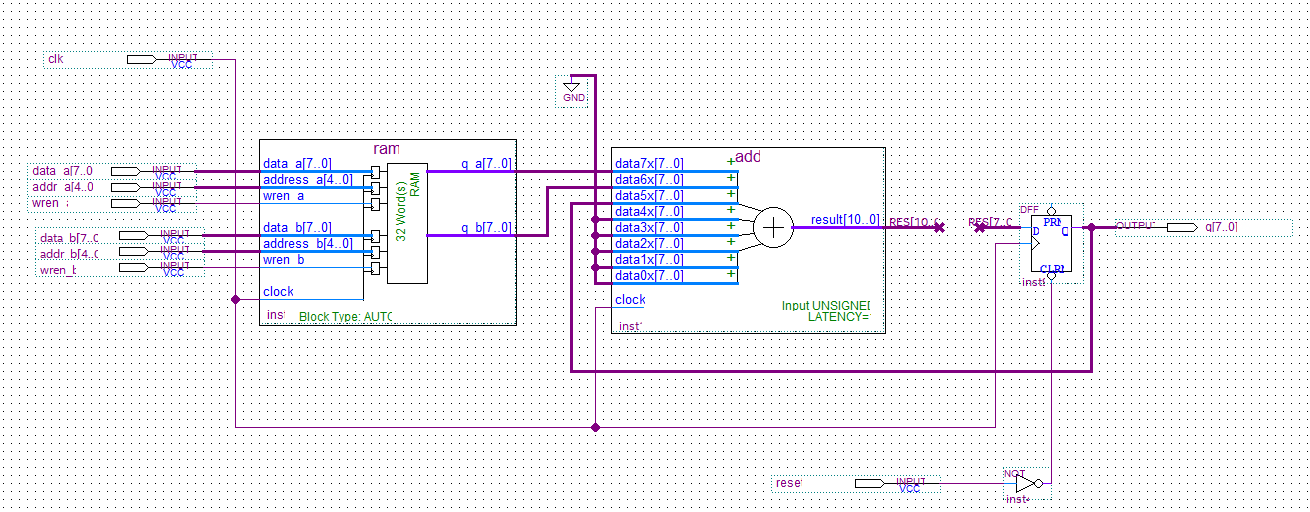
\includegraphics[width=\linewidth]{image/schema}
	\caption{Схема проекта}
	\label{fig:schema}
\end{figure}

Выполним компиляцию проекта.
В отчете компиляции (рис.~\ref{fig:report}) видно потребление логических и других элементов данным проектом.
Отчет о потреблении элементов на блок представлен на рис.~\ref{fig:elements}

\begin{figure}[H]
	\centering
	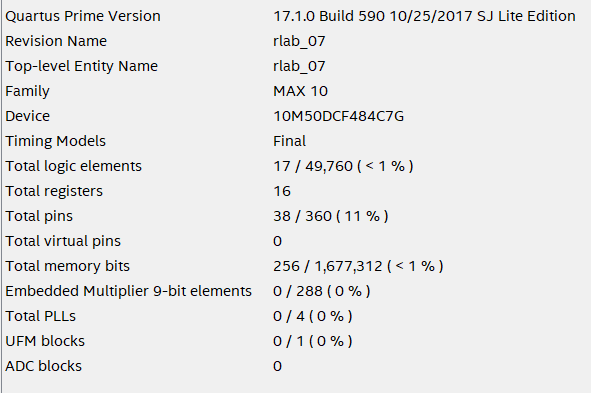
\includegraphics[width=0.6\linewidth]{image/report}
	\caption{Результат компиляции}
	\label{fig:report}
\end{figure}

\begin{figure}[H]
	\centering
	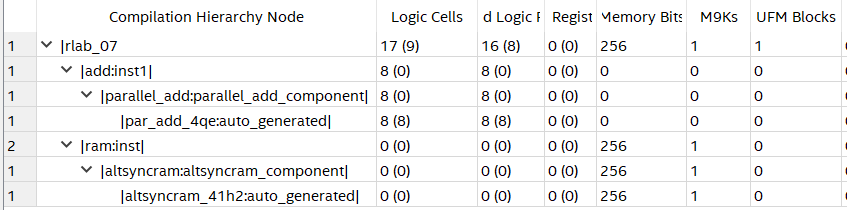
\includegraphics[width=0.6\linewidth]{image/elements}
	\caption{Потребление элементов}
	\label{fig:elements}
\end{figure}

Выполним тестирование схемы с помощью waveform.
На вход сумматора подаются попеременно пары чисел 1, 1 и 1, 3(рис.~\ref{fig:wave}).
Как можно заметить, результат суммирования увеличивается на 2 или 4 в зависимости от входных значений.
При подаче сигнала сброса результат вычислений выставляется в 0.

\begin{figure}[H]
	\centering
	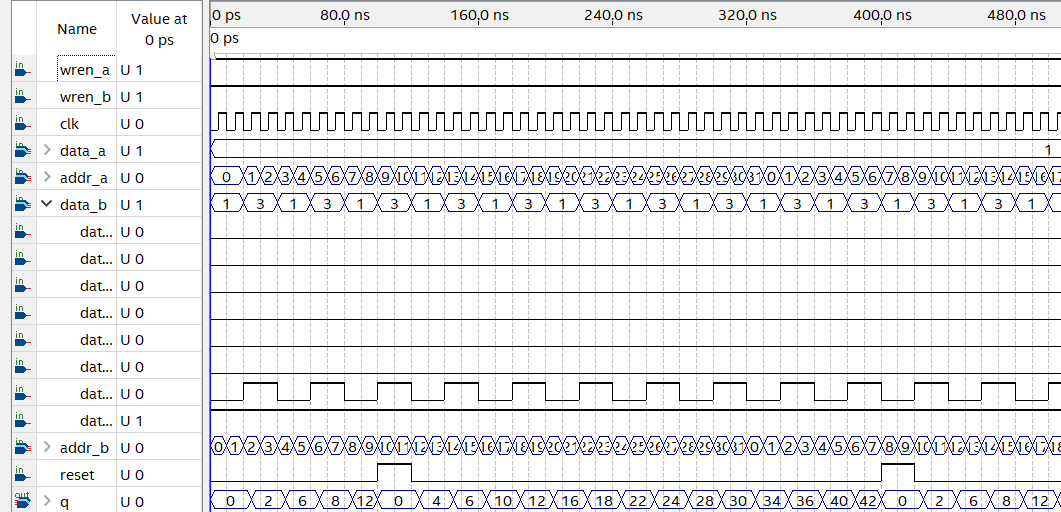
\includegraphics[width=\linewidth]{image/wave}
	\caption{Тестирование схемы}
	\label{fig:wave}
\end{figure}

Построим RTL представление проекта (рис.~\ref{fig:rtl}).

\begin{figure}[H]
	\centering
	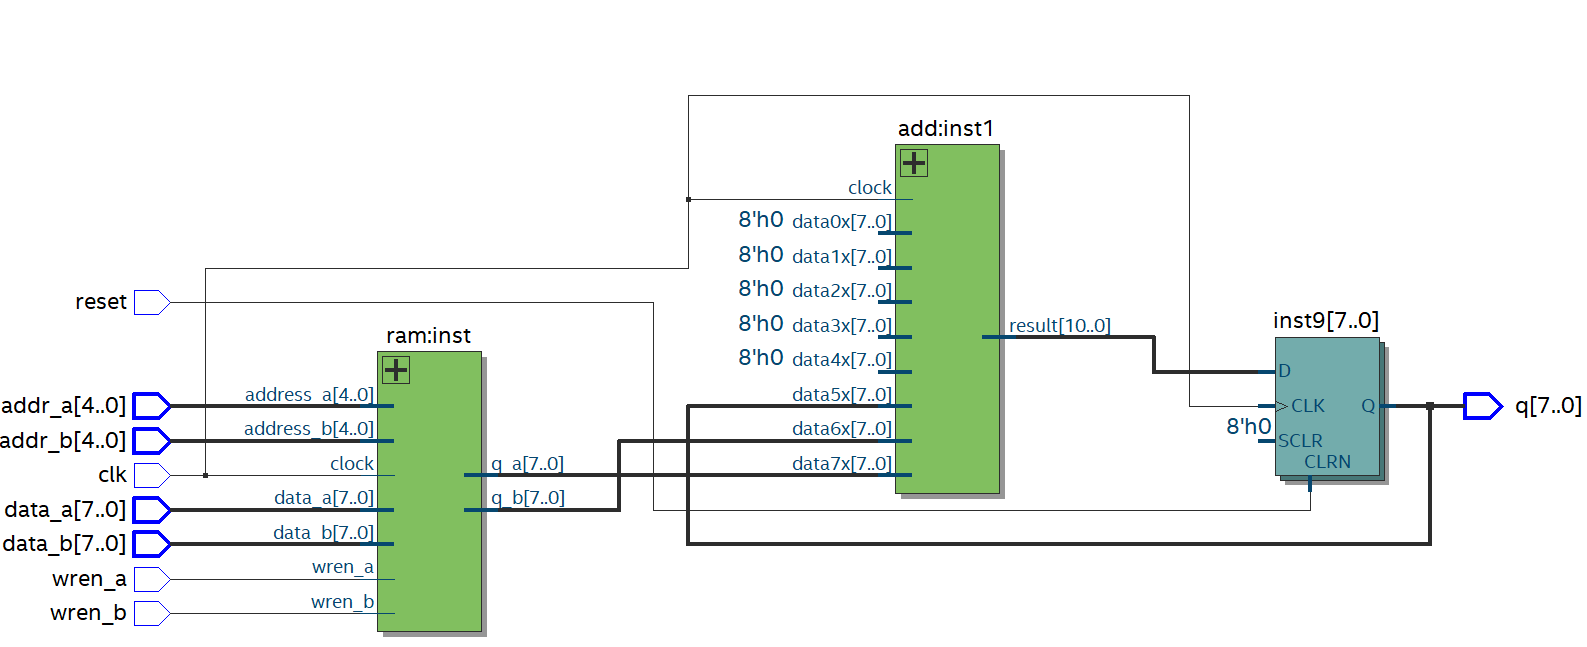
\includegraphics[width=\linewidth]{image/rtl}
	\caption{RTL представление проекта}
	\label{fig:rtl}
\end{figure}

Из RTL представления проекта перейдем в TMV представление памяти (рис.~\ref{fig:tmv}).

\begin{figure}[H]
	\centering
	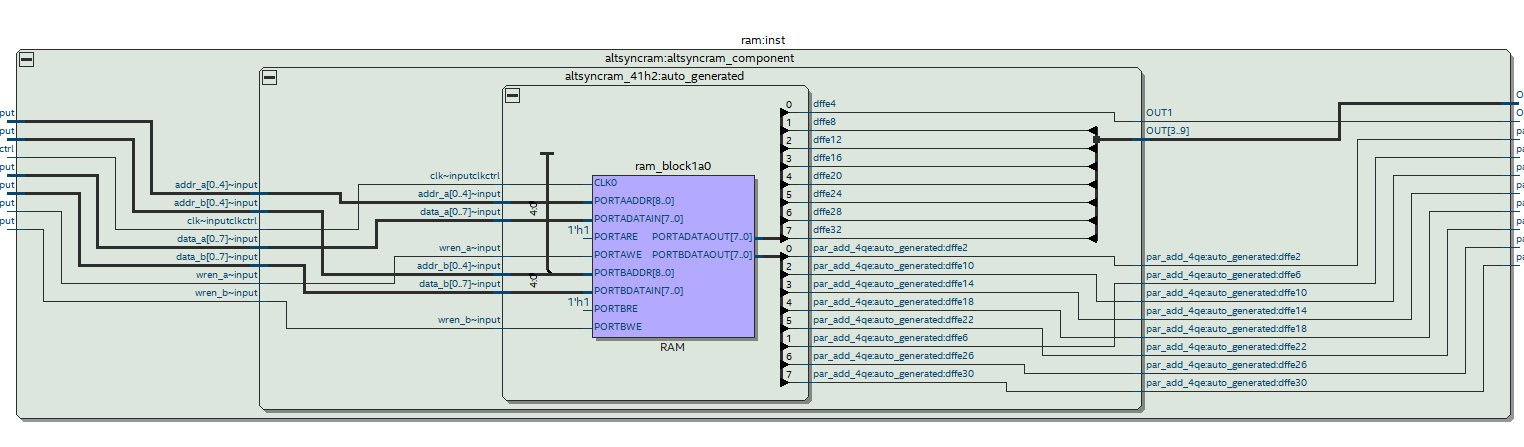
\includegraphics[width=\linewidth]{image/tmv}
	\caption{TMV представление памяти}
	\label{fig:tmv}
\end{figure}

Далее перейдем в chip planner и рассмотрим подробно входы (рис.~\ref{fig:mem_in}) и выходы (рис.~\ref{fig:mem_out}) памяти.

\begin{figure}[H]
	\centering
	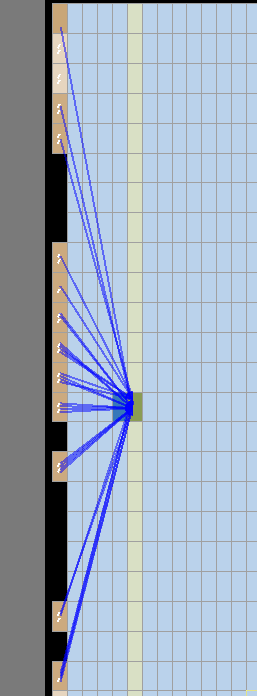
\includegraphics[width=0.3\linewidth]{image/mem_in}
	\caption{Входы в память}
	\label{fig:mem_in}
\end{figure}

\begin{figure}[H]
	\centering
	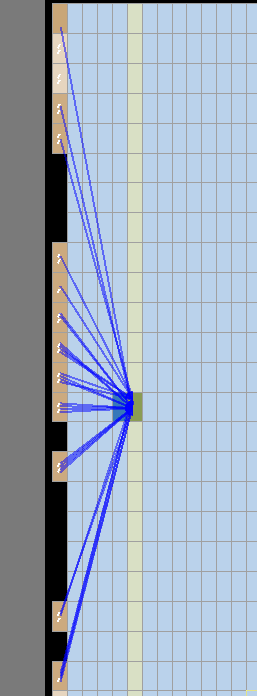
\includegraphics[width=0.3\linewidth]{image/mem_out}
	\caption{Выходы памяти}
	\label{fig:mem_out}
\end{figure}

Расположим пины по банкам, используемые в проекте пины подсвечены зеленым (рис.~\ref{fig:pins}).

\begin{figure}[H]
	\centering
	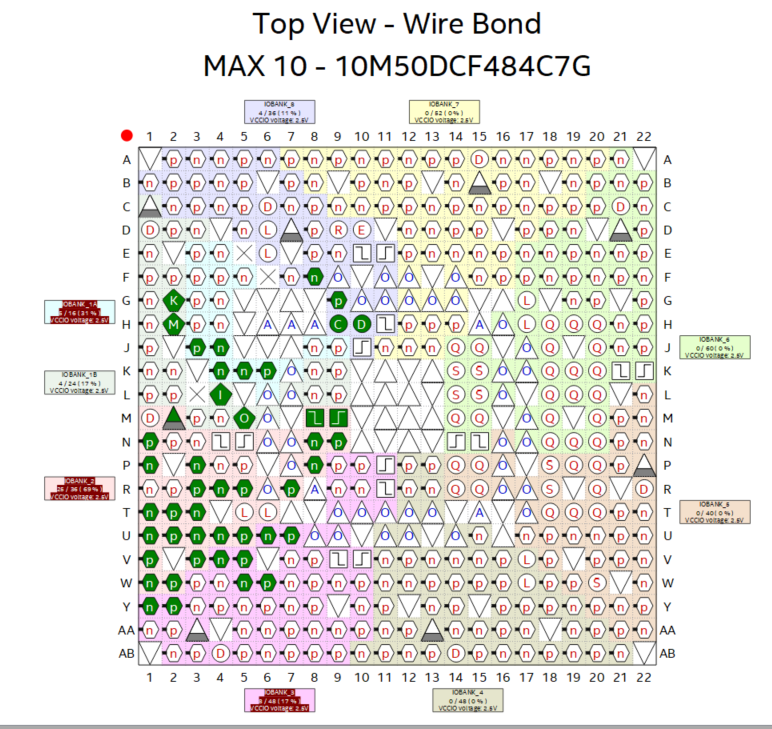
\includegraphics[width=0.8\linewidth]{image/pins}
	\caption{Назначение пинов}
	\label{fig:pins}
\end{figure}

Создадим новую ревизию проекта, настроим ее на оптимизацию энергопотребления (рис.~\ref{fig:settings}).
Выполним повторную сборку проекта, посмотрим на различия ревизий (рис.~\ref{fig:diff}).

\begin{figure}[H]
	\centering
	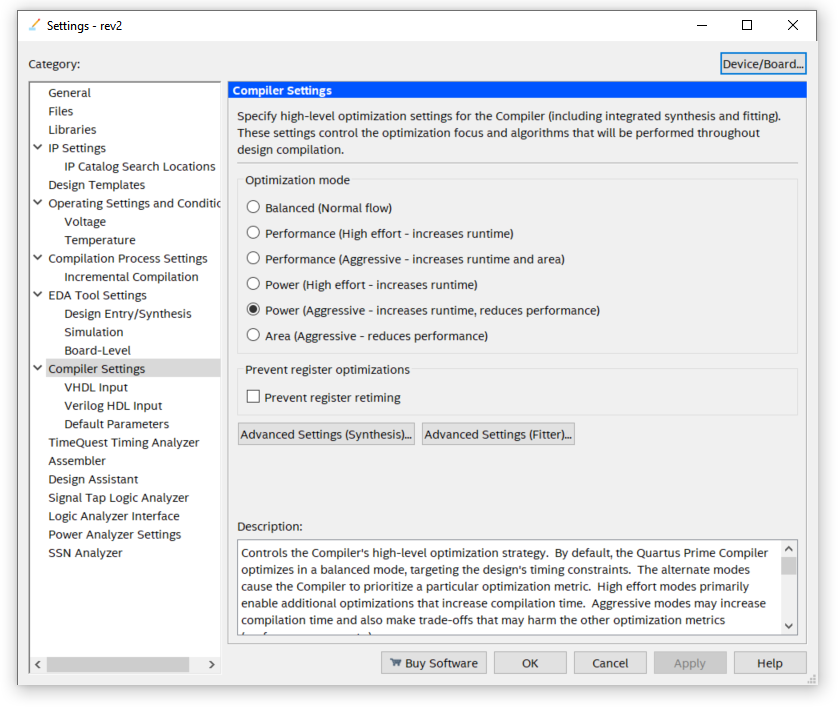
\includegraphics[width=0.8\linewidth]{image/settings}
	\caption{Настройка новой ревизии}
	\label{fig:settings}
\end{figure}

\begin{figure}[H]
	\centering
	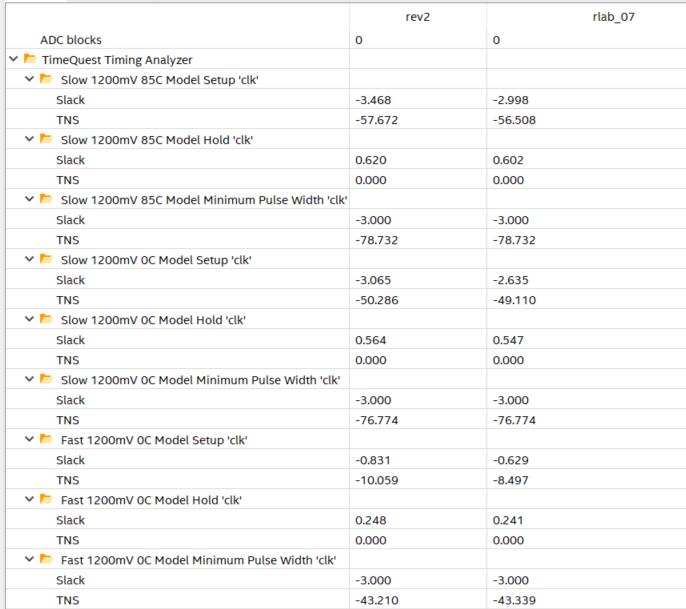
\includegraphics[width=0.8\linewidth]{image/diff}
	\caption{Сравнение ревизий}
	\label{fig:diff}
\end{figure}

\subsection{Демонстрация работы}

Была создана дополнительная оболочка для тестирования схемы на плате (рис.~\ref{fig:demo_schema}).
Было произведено тестирование на плате (рис.~\ref{fig:demo_1}~и~\ref{fig:demo_2}).

\begin{figure}[H]
	\centering
	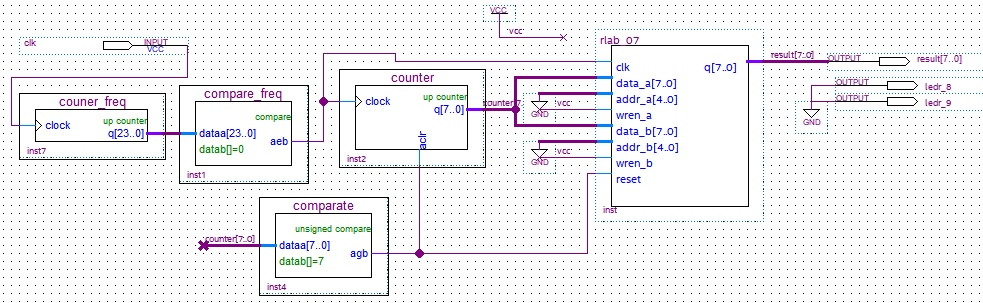
\includegraphics[width=\linewidth]{image/demo_schema}
	\caption{Схема для демонстрации}
	\label{fig:demo_schema}
\end{figure}

\begin{figure}[H]
	\centering
	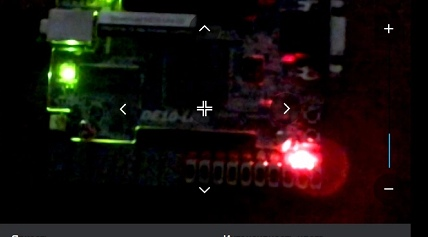
\includegraphics[width=0.8\linewidth]{image/demo_1}
	\caption{Демонстрация работы}
	\label{fig:demo_1}
\end{figure}

\begin{figure}[H]
	\centering
	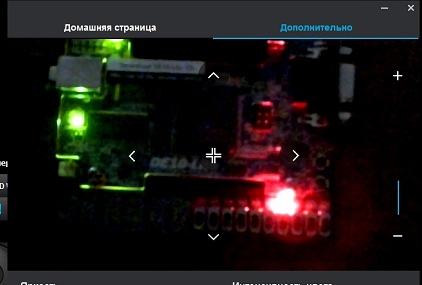
\includegraphics[width=0.8\linewidth]{image/demo_2}
	\caption{Демонстрация работы}
	\label{fig:demo_2}
\end{figure}

\section{Выводы по работе}

В ходе работы был получен блок накопительного сложения чисел с возможностью сброса результата.
Устройство были протестированы с помощью Quartus waveform, что подтвердило правильность работоспособности устройства.
Так же было выполнено построение RTL и TMV диаграмм для устройства, построены зависимости в chip planer, настроены пины.

\newpage 
\renewcommand{\refname}{{\normalsize Список использованных источников}} 
\centering 
\begin{thebibliography}{9} 
	\addcontentsline{toc}{section}{\refname} 
	\bibitem{Verilog} Thomas D., Moorby P. The Verilog Hardware Description Language. – Springer Science \& Business Media, 2008.
	\bibitem{Quartus} Антонов А., Филиппов А., Золотухо Р. Средства системной отладки САПР Quartus II //Компоненты и технологии. – 2008. – №. 89.
\end{thebibliography}

\end{document} % конец документа